% Compile with XeLaTeX or LuaLaTeX for fontspec support
\documentclass{article}

\usepackage{arxiv}
\usepackage{fontspec}
\setmainfont{Linux Libertine O}
% \setmainfont{Inter}

\usepackage{polyglossia}
\setdefaultlanguage{english}
\setotherlanguage{russian}

\usepackage{url}
\usepackage{booktabs}
\usepackage{amsfonts, amssymb, amsmath, amsthm}
\usepackage{nicefrac}
\usepackage{microtype}
\usepackage{graphicx}
\usepackage{forest}

\usepackage{mathtools}
\usepackage{xcolor}
\usepackage{doi}
\usepackage{caption}

\usepackage[backend=biber, style=authoryear]{biblatex}
\addbibresource{references.bib}

\usepackage{ragged2e}
\usepackage{braket}
\usepackage[colorinlistoftodos]{todonotes}

% Custom TODO commands
\newcommand{\todoask}[1]{\todo[color=blue!30]{\textbf{Ask:} #1}}
\newcommand{\todocheck}[1]{\todo[color=green!30]{\textbf{Check:} #1}} 
\newcommand{\todoread}[1]{\todo[color=orange!30]{\textbf{Read:} #1}} 
\newcommand{\todocomment}[1]{\todo[color=purple!30]{\textbf{Comment:} #1}}

%% ============================================================================================================
%% Math commands and symbols
%% ============================================================================================================
\newcommand{\RMSE}[2]{\operatorname{RMSE}{\left(#1, #2\right)}}
\newcommand{\MAE}[2]{\operatorname{MAE}{\left(#1, #2\right)}}
\newcommand{\MAPE}[2]{\operatorname{MAPE}{\left(#1, #2\right)}}
\newcommand{\NSE}[2]{\operatorname{NSE}{\left(#1, #2\right)}}

\DeclareMathOperator*{\argmax}{arg\,max}
\DeclareMathOperator*{\argmin}{arg\,min}

\newcommand{\Indicator}[1]{\mathbf{1}_{\set{#1}}}
\newcommand{\SetPower}[1]{\##1}

\newcommand{\Reals}{\mathbb{R}}

\newcommand{\Ell}{\mathcal{L}}
\newcommand{\Dataset}{\mathcal{D}}
\newcommand{\Models}{\mathcal{F}}
\newcommand{\Model}{\hat{f}}
\newcommand{\BestModel}{f^*}


%% ============================================================================================================
%% Metadata
%% ============================================================================================================
\title{Comparative Analysis of Data-Driven Approaches for Hydrological Forecasting}

\author{
    Eldar Khuzin \\
    Chair of Data Analysis\\
    Moscow Institute of Physics and Technology\\
    Moscow, Russia \\
    \texttt{khuzin.er@phystech.su} \\
    \And
    Novikov Ivan \\
    Affiliation \\
    Address \\
    \texttt{email} \\
    \AND
    Abramov Dmitrii \\
    Affiliation \\
    Address \\
    \texttt{email}
}

\date{}

\hypersetup{
    pdftitle={Comparative Analysis of Data-Driven Approaches for Hydrological Forecasting},
    pdfsubject={cs.LG},
    pdfauthor={Eldar Khuzin, Novikov Ivan, Abramov Dmitrii},
    pdfkeywords={Flood discharge, Rainfall-runoff modeling, More}
}

%% ============================================================================================================
%% Document begin
%% ============================================================================================================
\begin{document}
\sloppy
\justifying

\maketitle

\begin{abstract}
    In this article, we address the problem of equifinality in data-driven hydrological modeling — when different feature sets or model architectures yield similar predictive efficiency. We investigate the influence of static catchment features on predictions made by traditional models, recurrent neural networks, and transformers across various river basins in Eurasia. By analyzing feature importance and model behavior, we identify dominant predictors and assess the practicality of employing complex models in terms of interpretability and computational cost. This approach provides insights into the trade-offs between model complexity and predictive robustness in the presence of equifinality.
\end{abstract}


\keywords{Flood discharge \and Rainfall-runoff modeling \and More}

\listoftodos[List of suggested changes]

%% ============================================================================================================
%% Introduction
%% ============================================================================================================
\section{Introduction}
\label{sec:introduction}

\todo[inline]{Add models from the problem statment section as ``Quantile Random Forest (QRF)'', ``Gradient‑Boosted Trees (GBT)'' and so on.}

%% ============================================================================================================
%% Problem Statement
%% ============================================================================================================
\section{Problem Statement}
\label{sec:problem-statement}

\paragraph{Notation}
\begin{itemize}
    \item Let \(y \in \Reals^n\) and \( y_i \in \Reals \) denote target; \(x \in \Reals^{n \times d}\) and \( x_i \in \Reals^d \) denote \(d\) features associated with \( y_i \), where \(n\) is the number of samples;
    \item Let the dataset be \( \Dataset = \set{(x_i, y_i) \mid i \in \overline{1, n}} \) --- set of \(n\) pairs for features and targets.
    \item Let the models class be denoted as \(\Models\);
    \item Let \( \hat{y}_i \coloneqq f(x_i),\, f \in \Models\) denotes estimation of \( y_i \) based on \( x_i \);
    \item Let assume \(\hat{y} \coloneqq \left( \hat{y}_1, \dots, \hat{y}_n \right) = \left( f(x_1), \dots, f(x_n) \right)\).
\end{itemize}


% Optimization statement
% ————————————————————————————————————————————————————————————————————————————
\subsection{Optimization statement}

In general, in each experiment we find the optimal model \(\BestModel\) s.t.

\begin{equation}
    \BestModel
    =
    \argmin\limits_{f \in \Models}{\left( \Ell(f, \Dataset) + \Omega(f) \right)},
    \label{oprimization:general-task}
\end{equation}

where:

\begin{itemize}
    \item \( \Ell(f, \Dataset) \) denotes the empirical loss of model \(f\) on dataset \(\Dataset\);
    \item \( \Omega(f) \) is a regularization term penalizing model complexity.
\end{itemize}

Let \(\ell(\cdot, \cdot)\) denotes the actual loss function, so \(\Ell(f, \Dataset) = \ell(y, \hat{y}) = \frac{1}{n}{\sum\limits_{i=1}^{n}{\ell(y_i, \hat{y}_i)}} \).

In our work we choose\todo{Link to article and explanation why MAPE} \(\ell\) as a mean absolute percentage error (\ref{metric:mape}), so \ref{oprimization:general-task} can be rewriten as

\begin{equation}
    \BestModel
    =
    \argmin\limits_{
        f \in \Models
    }{
        \left(
        \sum_{i=1}^{n} \left| \frac{y_i - f({x_i})}{y_i} \right|
        +
        \Omega(f)
        \right)
    }.
    \label{oprimization:task}
    \tag{Opt.~task}
\end{equation}

% ————————————————————————————————————————————————————————————————————————————
% End of 'Optimization statement'


% Model's description
% ————————————————————————————————————————————————————————————————————————————
\subsection{Model's descriptions}

% Regression trees
% ------------------------------------------------------
\subsubsection{Regression trees}\todo{Add link to article, where trees were presented}
\label{model:regression-tree}

In some experiments we use regression trees as base predictors. In general, regression tree is binary tree, which can be written as
\begin{equation}
    f(x)
    =
    \sum\limits_{l=1}^{L}\Indicator{x \in R_l}\cdot\omega_l,
\end{equation}
where:
\begin{itemize}
    \item \(R_l,\, l \in \overline{1, L}\) form a partition of \(\Reals^d\) into disjoint sets;
    \item \(\omega_l\) are constant weights on tree leaves.
\end{itemize}

To perform the partitioning into \( R_l \), each node of the binary tree acts as a simple predicate of the form \( x^{(j)} \le t \), used to select between the left and right child. Here, \( x^{(j)} \) denotes a coordinate in the features \( \Reals^d \) space, and \( t \) is a \emph{threshold}.

\todo[inline]{Add a picture of three}

To select a threshold \( t \) and the corresponding feature index \( j \) at each node, the algorithm maximizes an objective function known as the \emph{information gain (IG, \(\mathcal{IG}\))}. We are going to use the same IG as \cite{chenXGBoostScalableTree2016a}. Let assume \(\hat{y}_i^{(0)}\) as initial prediction (constant)\todo{Think about initial value.}:
\[
    \mathcal{IG}(t, j)
    =
    \frac{1}{2}
    \left[
        \frac{\left(\sum_{i\in \mathcal{I}_L} g_i\right)^2}{\sum_{i\in \mathcal{I}_L} h_i + \lambda}
        +
        \frac{\left(\sum_{i\in \mathcal{I}_R} g_i\right)^2}{\sum_{i\in \mathcal{I}_R} h_i + \lambda}
        -
        \frac{\left(\sum_{i\in \mathcal{I}} g_i\right)^2}{\sum_{i\in \mathcal{I}} h_i + \lambda}
        \right]
    -
    \gamma,
\]
where:
\begin{itemize}
    \item \(\mathcal{I}_L = \{\,i: x_{i}^{(j)} \le t\}\) --- indices, which are going to be in the left child if node use threshold \(t\) and feature \(j\);
    \item \(\mathcal{I}_R = \{\,i: x_{i}^{(j)} > t\}\) --- same, but in the right child;
    \item \(g_i = \left.\frac{\partial \ell(y_i, \hat{y}_i)}{\partial \hat{y}_i}\right|_{\hat y_i = \hat{y}_i^{(0)}}\) and
          \(h_i = \left.\frac{\partial^2 \ell(y_i, \hat{y}_i)}{\partial \hat{y}_i^2}\right|_{\hat y_i = \hat{y}_i^{(0)}}\) are the first and second derivatives of the loss;
    \item \(\lambda\) is the \(L_2\) regularization weight on leaf scores;
    \item \(\gamma\) is the complexity penalty for adding a new leaf.
\end{itemize}

In other words, we find a best split in node for \ref{oprimization:task} where complexity penalizes is \(\Omega(f) = \gamma{L} + \frac{1}{2}\lambda\| w \|^2_2\)

Then, once the tree structure is fixed, we assign each leaf \(l\) the weight
\[
    \omega_l
    =
    -\frac{G_l}{H_l + \lambda},
    \quad
    \text{where }
    G_l = \sum_{i \in R_l} g_i,
    H_l = \sum_{i \in R_l} h_i.
\]
% ------------------------------------------------------
% End of 'Regression trees'

% Random Forest
% ------------------------------------------------------
\subsubsection{Random Forest}
\label{model:random-forest}

Random Forest (RF) is an ensemble of \(B\) regression trees\cite{breimanRandomForests2001}, each trained on a bootstrap draw of the training set. At every split, instead of scanning all \(d\) features, only a random subset of \(m_{\mathrm{try}}\ll d\) candidates is used. Thus, each tree \(f^{(i)}\) is both bagged and feature-subsampled, and the RF prediction is

\begin{equation}
    f(x)
    =
    \frac{1}{B}\sum_{I=1}^B f^{(i)}(x).
\end{equation}

This dual randomness (bagging + feature subsampling) (1) lowers variance by averaging many decorrelated trees, and (2) secure from overfitting despite fully grown leaves.

Primary hyperparameters:
\begin{itemize}
    \item \(B\) --- number of trees;
    \item \(m_{\mathrm{try}}\) --- (features per split);
    \item ``Bootstrap sample size'' --- \(n\) draws with replacement.
\end{itemize}

\cite{breimanRandomForests2001} showed that as \(B \to \infty\), RF variance go to zero if trees correlation is lowest.
% ------------------------------------------------------
% End of 'Random Forest'


%%% ************************
%%% % Quantile Random Forest
%%% % ------------------------------------------------------
%%% \subsubsection{Quantile Random Forest}
%%% Followed the \cite{meinshausenQuantileRegressionForests2006} we build a quantile random forest (QRF) on ensemble of \ref{model:regression-tree}.
%%% % ------------------------------------------------------
%%% % End of 'Quantile Random Forest'
%%% ************************

% Gradient Boosting
% ------------------------------------------------------
\subsubsection{Gradient Boosting}
\label{model:gradient-boosting}

Gradient Boosting (also called Gradient Boosting Machine, GBM) \cite{friedmanGreedyFunctionApproximation2001} builds an additive ensemble of \(B\) regression trees by successive error correction. Starting from an initial guess \(f^{(0)}(x)\), each new tree \(h^{(b)}\) is fit to the negative gradient (residuals) of the loss \(\ell\) with respect to the current model. Formally, GBM is

\begin{equation}
    f_{(B)}(x) = f^{(0)} + \nu\sum\limits_{i=1}^{B}{f^{(i)}(x)},
\end{equation}

where

\begin{itemize}
    \item \(\nu\) --- is a learing rate hyperparameter;
    \item \(B\) --- number of trees;
    \item \(f^{(b)}\) --- regression tree;
\end{itemize}

and each of the tree is trained to predict the errors of the previous state model \(f_{(B-1)}\):

\begin{equation}
    f^{(B)} = \argmin\limits_{f\in\Models}{\sum_{i=1}^{n}{\ell(y_i - f_{(B-1)}(x_i), f(x_i))}}
\end{equation}

% ------------------------------------------------------
% End of 'Gradient Boosting'

% SARIMA
% ------------------------------------------------------
\subsubsection{SARIMA}
\label{model:sarima}

Seasonal Autoregressive (AR) Integrated Moving Average (MA) (SARIMA) is the extention of ARIMA model (combination of SARIMA).

Let's denotes
\begin{itemize}
    \item \(L\) --- back‑shift (lag) operator, means \(L\,y_{t}=y_{t-1}\);
    \item \(a(L)=1-a_{1}L-\dots-a_{p}L^{p}\) (AR polynomial);
    \item \(b(L)=1-b_{1}L-\dots-b_{q}L^{q}\) (MA polynomial);
    \item \(d\) --- number of non‑seasonal differences needed for stationarity.
\end{itemize}

% ARIMA
% . . . . . . . . . . . . . .
\paragraph{ARIMA \texorpdfstring{\((p,d,q)\)}{(p,d,q)}}

\begin{equation}
    (1-L)^{d}\,y_{t} = \mu + \frac{b(L)}{a(L)}\,\varepsilon_{t},
\end{equation}
% . . . . . . . . . . . . . .
% ARIMA

% SARIMA
% . . . . . . . . . . . . . .
\paragraph{Add seasonality \texorpdfstring{\(\Rightarrow\)}{--- get} SARIMA
    \texorpdfstring{\((p,d,q)\!\times\!(P,D,Q)_{s}\)}{(p,d,q) x (P,D,Q)\_s}}

\begin{equation}
    (1-L)^{d}(1-L^{s})^{D}\,y_{t} =
    \mu +
    \frac{b(L)\,B(L^{s})}{a(L)\,A(L^{s})}\,\varepsilon_{t},
\end{equation}
where
\begin{itemize}
    \item \(s\) — seasonal period;
    \item \((P,D,Q)\) — AR, differencing, and MA orders of the \emph{seasonal} component:
          \begin{itemize}
              \item \(A(L) = 1 - A_1\,L^{s} - A_2\,L^{2s} - \cdots - A_P\,L^{Ps}\);
              \item \(B(L) = 1 - B_1\,L^{s} - B_2\,L^{2s} - \cdots - B_Q\,L^{Qs}\).
          \end{itemize}
\end{itemize}
% . . . . . . . . . . . . . .
% SARIMA

% ------------------------------------------------------
% End of 'SARIMA'

% ————————————————————————————————————————————————————————————————————————————
% End of 'Model's description'

% Metrics descriptions
% ————————————————————————————————————————————————————————————————————————————
\subsection{Evaluation Metrics Used}

\paragraph{Notation}
\begin{itemize}
    \item \( n \) is the total number of observations;
    \item \( y_i \) denotes the value for the \( i \)-th observation;
    \item \( \widehat{y}_i \) denotes the model estimation value for the \( i \)-th observation based on features \( x_i \);
    \item \( \overline{y} \) is the sample mean.
\end{itemize}

\paragraph{Root Mean Squared Error (RMSE)}
\begin{equation}
    \RMSE{y}{\widehat{y}} = \sqrt{\frac{1}{n} \sum_{i=1}^{n} \left(y_i - \widehat{y}_i\right)^2}.
    \label{metric:rmse}
    \tag{RMSE}
\end{equation}

\paragraph{Mean Absolute Error (MAE)}
\begin{equation}
    \MAE{y}{\widehat{y}} = \frac{1}{n} \sum_{i=1}^{n} \left|y_i - \widehat{y}_i\right|.
    \label{metric:mae}
    \tag{MAE}
\end{equation}

\paragraph{Mean Absolute Percentage Error (MAPE)}
\begin{equation}
    \MAPE{y}{\widehat{y}}
    = \frac{1}{n} \sum_{i=1}^{n} \left| \frac{y_i - \widehat{y}_i}{y_i} \right| \cdot 100\%.
    \label{metric:mape}
    \tag{MAPE}
\end{equation}

\paragraph{Nash-Sutcliffe Efficiency (NSE)}
Originally developed in hydrology, the NSE evaluates the predictive power of hydrological models.
\begin{equation}
    \NSE{y}{\widehat{y}} = 1 - \frac{\sum_{i=1}^{n} \left( y_i - \widehat{y}_i \right)^2}{\sum_{i=1}^{n} \left( y_i - \overline{y} \right)^2}.
    \label{metric:nse}
    \tag{NSE}
\end{equation}

\subparagraph{Interpretation:}
\begin{itemize}
    \item NSE \( = 1 \) indicates a perfect match between model and observations.
    \item NSE \( = 0 \) implies that the model is no better than using the mean of the observed data.
    \item NSE \( < 0 \) suggests the model predictions are worse than the mean.
\end{itemize}

%% ============================================================================================================
%% Methodology
%% ============================================================================================================
\section{Methodology}
\label{sec:methodology}

\subsection{Correlation analysis}
\todo{Describe the idea}
% \begin{figure}[htbp]
%     \centering
%     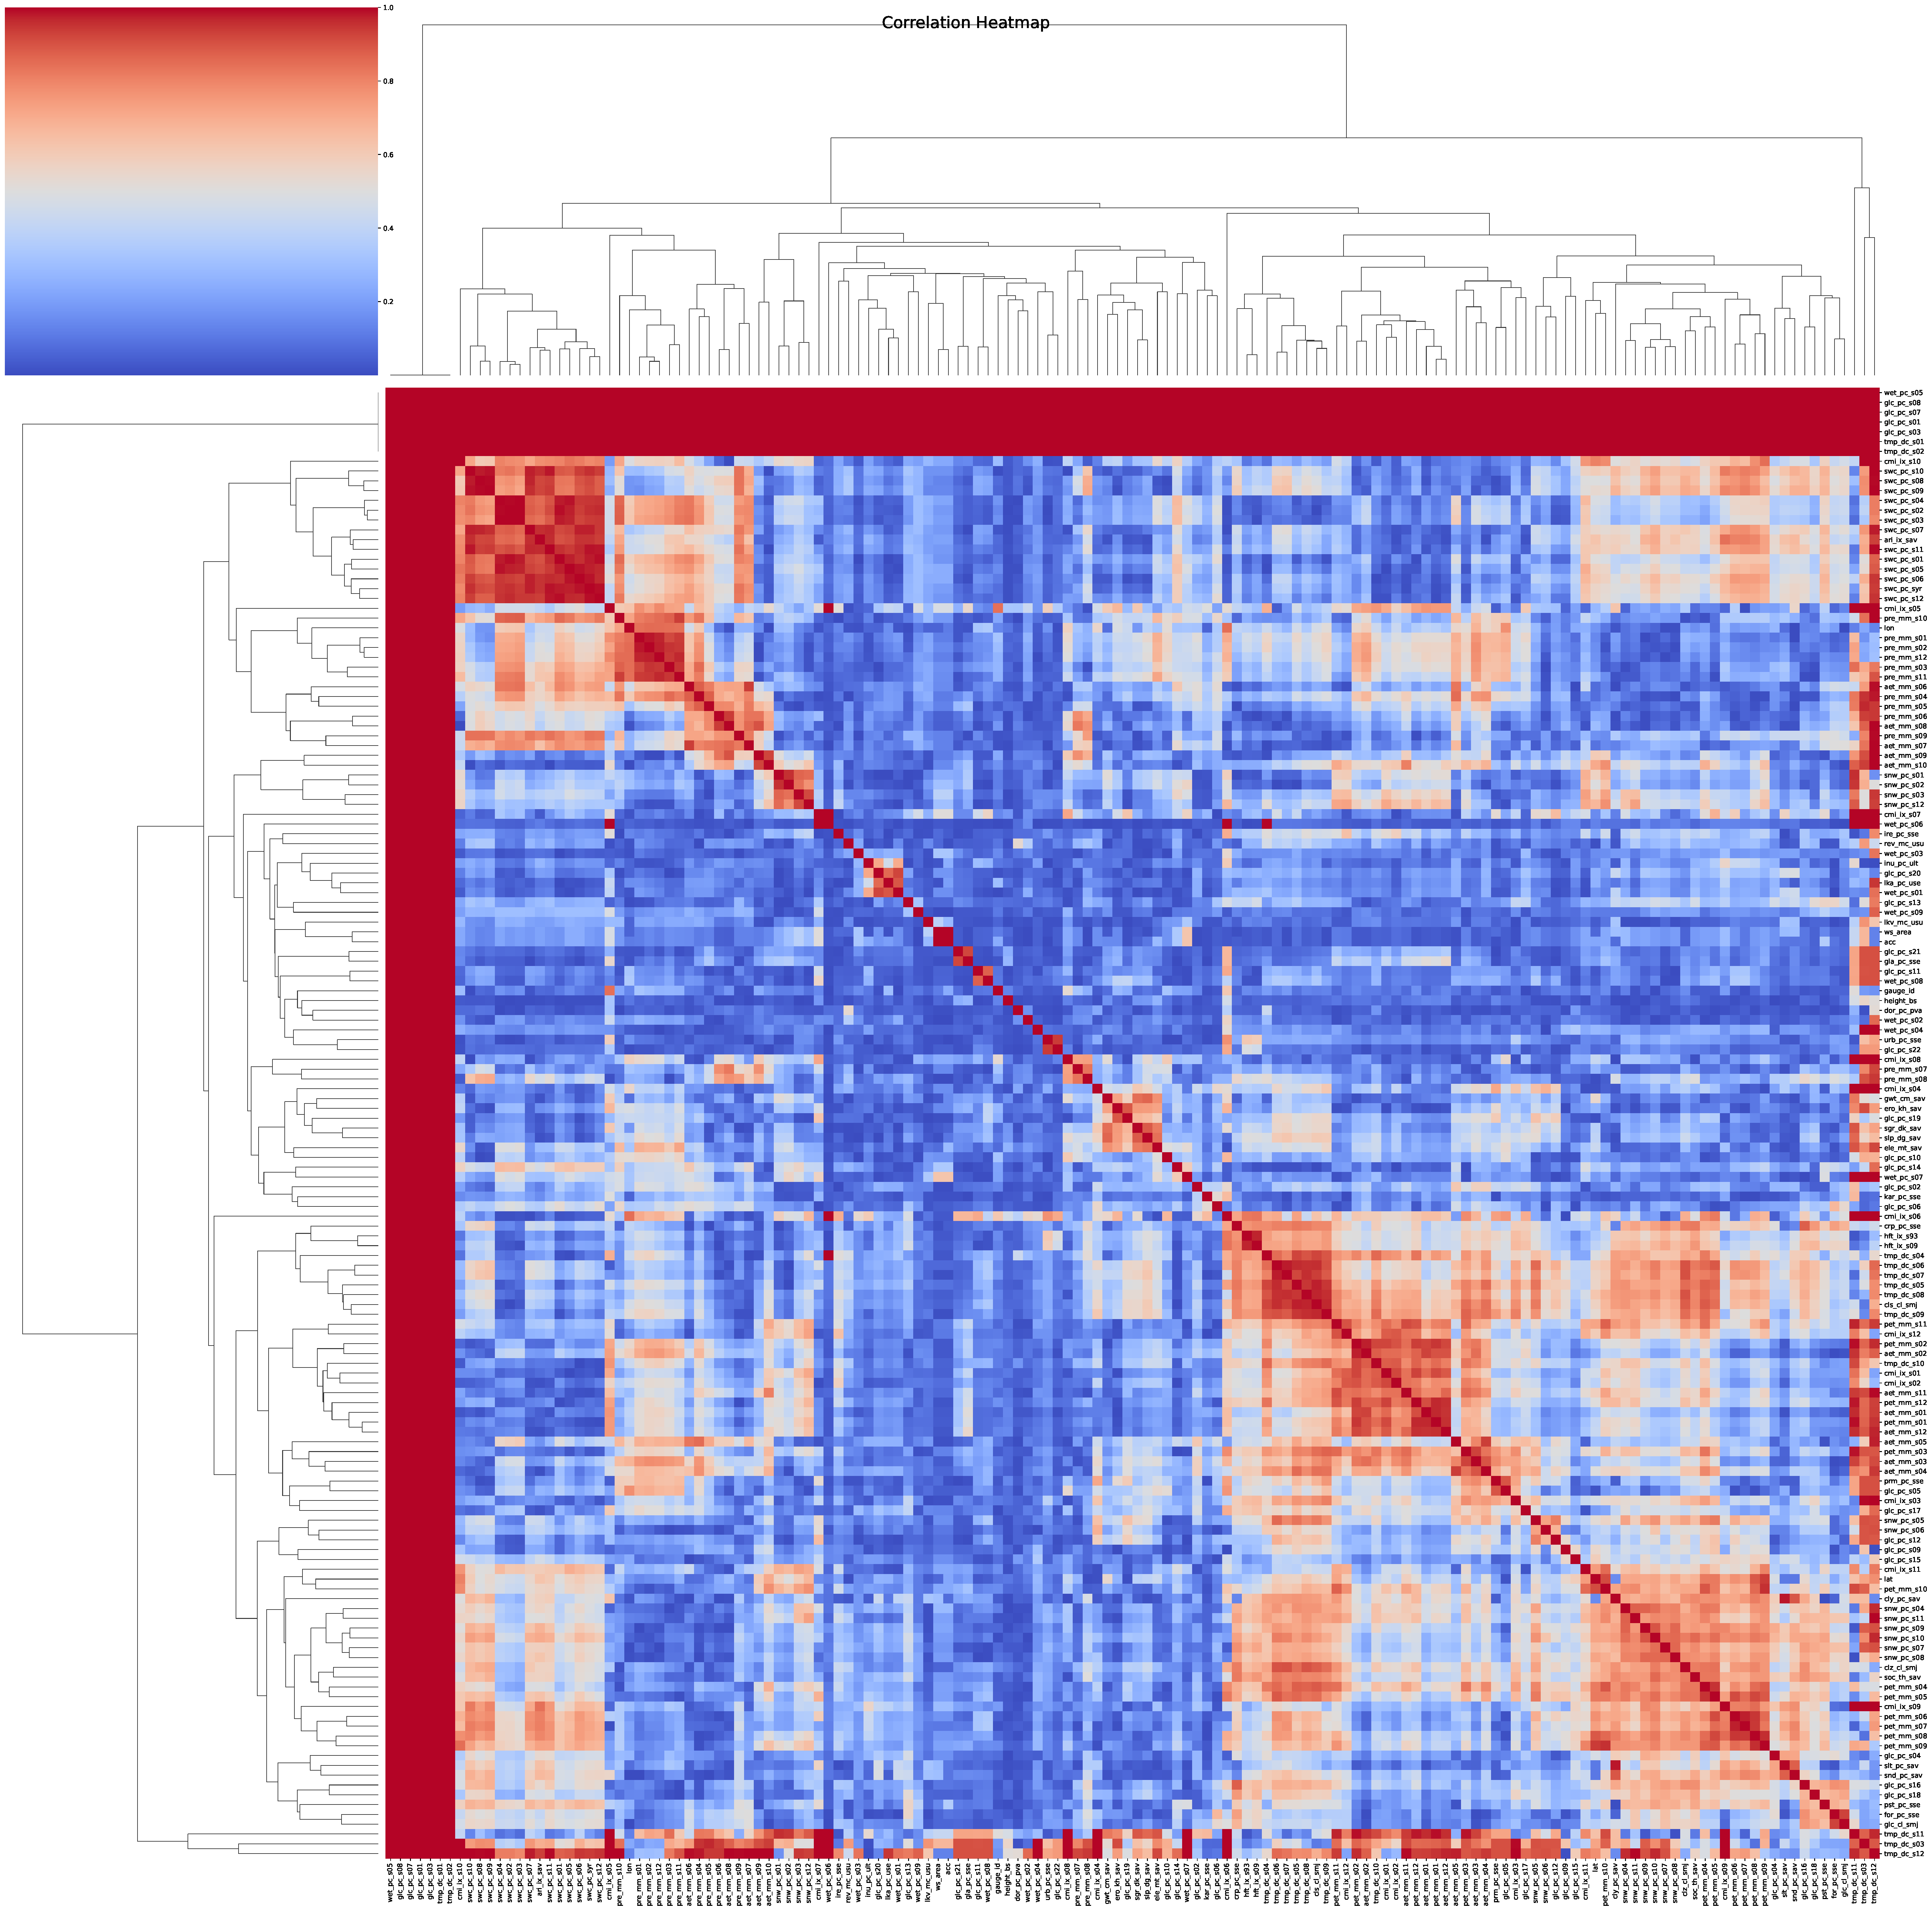
\includegraphics[width=\linewidth]{bin/static_features_heatmap.pdf}
%     \caption{Correlation analysis between the static features.}
%     \label{fig:correlation-analysis-static-features}
% \end{figure}

%% ============================================================================================================
%% Computational experiment
%% ============================================================================================================
\section{Computational experiment}
\label{sec:computational-experiment}

% Software
% ————————————————————————————————————————————————————————————————————————————
\subsection*{Software}
% \begin{refcontext}[style=numeric]
All experiments were conducted in Python 3.12 using the following open-source libraries:
\begin{itemize}
    \item \texttt{scikit-learn} (version *.*.*) for implementation of Random Forest models~\cite{pedregosaScikitlearnMachineLearning}.
    \item \texttt{XGBoost} (version *.*.*) for gradient boosting models~\cite{chenXGBoostScalableTree2016a}.
    \item \texttt{Dask} (version ) for parallel and distributed computation~\cite{rocklinDaskParallelComputation2015}.
    \item \texttt{NumPy} and \texttt{Pandas} for data manipulation and preprocessing.
    \item \texttt{Matplotlib} and \texttt{Seaborn} for visualization.
\end{itemize}
Experiments were executed on a machine \todo{describe the machine}. The complete source code and environment configuration files are available at: \url{https://github.com/intsystems/2025-Project-188}.
% \end{refcontext}

% Datasets
% ————————————————————————————————————————————————————————————————————————————
\subsection*{Datasets}
\todo{todo}

\subsubsection*{Map}
\todo{todo}

\subsubsection*{Time series}
\todo{todo}

\subsubsection*{Static features}
\todo{todo}

% Experiment 1. QRF
% ————————————————————————————————————————————————————————————————————————————
\subsection{Experiment 1. Random Forest}
\label{experiment:random-forest}

% Experiment 2. GBRT
% ————————————————————————————————————————————————————————————————————————————
\subsection{Experiment 2. GBRT}
\label{experiment:GBRT}

% Experiment 3. LSTM
% ————————————————————————————————————————————————————————————————————————————
\subsection{Experiment 3. SARIMAX}
\label{experiment:SARIMAX}


% Experiment 4. LSTM
% ————————————————————————————————————————————————————————————————————————————
\subsection{Experiment 4. LSTM}
\label{experiment:LSTM}

%% ============================================================================================================
%% Results
%% ============================================================================================================
\section{Results}
\label{sec:results}

%% ============================================================================================================
%% Discussion
%% ============================================================================================================
\section{Discussion}
\label{sec:discussion}

%% ============================================================================================================
%% Conclusion
%% ============================================================================================================
\section{Conclusion}
\label{sec:conclusion}


%% ============================================================================================================
%% Notation
%% ============================================================================================================
\section*{Notations}

\begin{table}[h!]
    \centering
    \renewcommand{\arraystretch}{1.3}
    \begin{tabular}{llp{7cm}}  % Adjust width if needed
        \toprule
        \textbf{Symbol} & \textbf{Formula}                              & \textbf{Description} \\
        \midrule
        $\overline{x}$  & $\displaystyle\frac{1}{n} \sum_{i=1}^{n} x_i$
                        & Sample mean of the values $x_1, \dots, x_n$                          \\
        \bottomrule
    \end{tabular}
    \caption{Summary of frequently used symbols and their meanings.}
\end{table}


%% ============================================================================================================
%% Bibliography
%% ============================================================================================================
\printbibliography

\end{document}
